\documentclass[10pt]{article}
\usepackage[polish]{babel}
\usepackage[utf8]{inputenc}
\usepackage[T1]{fontenc}
\usepackage{graphicx}
\usepackage[export]{adjustbox}
\graphicspath{ {./images/} }
\usepackage{amsmath}
\usepackage{amsfonts}
\usepackage{amssymb}
\usepackage[version=4]{mhchem}
\usepackage{stmaryrd}

\title{X Konkurs matematyczny St@ś }

\author{XIV LO im. Stanisława Staszica\\
2 czerwca 2010 roku}
\date{}


\begin{document}
\maketitle


\section*{klasa V}
Na rozwiazanie poniższych zadań masz 90 minut.\\
Kolejność rozwiazywania tych zadań jest dowolna.\\
Wszystkie zadania sq jednakowo punktowane.\\
Maksymalnq liczbę punktów może uzyskać jedynie petne rozwiqzanie, z uzasadnieniem i odpowiedzia.\\
Użwanie korektora i korzystanie z kalkulatora jest niedozwolone.

\section*{Zadanie 1.}
Przerysuj tabelkę. W puste kratki wpisz takie liczby naturalne różne od dwójki, aby iloczyny liczb w każdym rzędzie poziomym i w każdym rzędzie pionowym były równe.\\
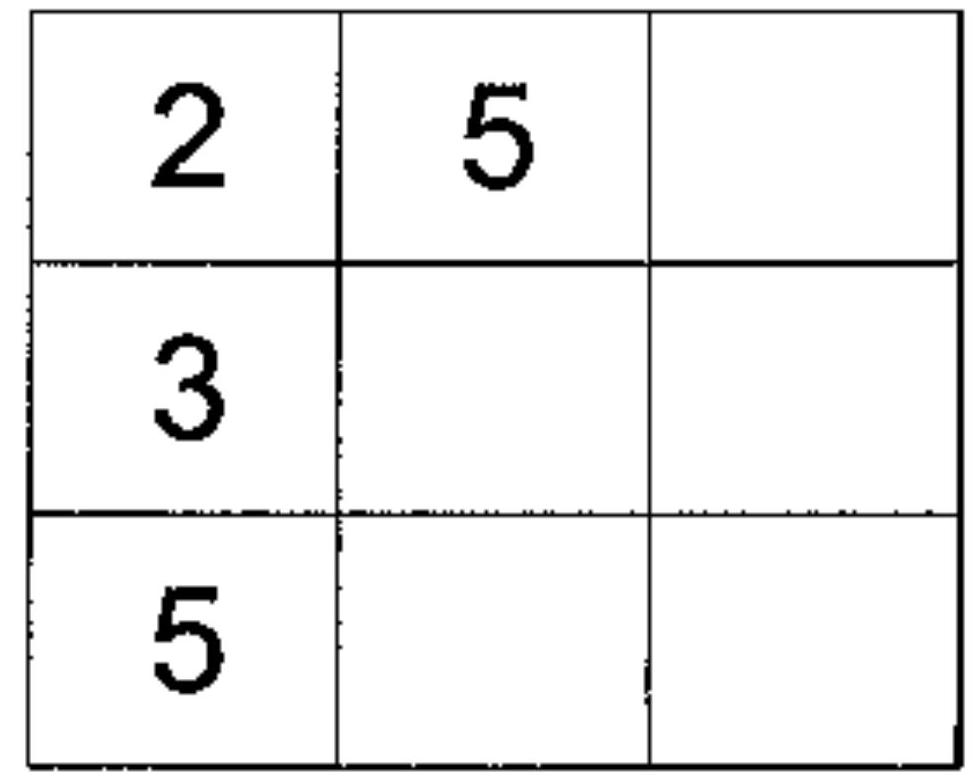
\includegraphics[max width=\textwidth, center]{2024_11_21_a3163903e65e7e4f74cag-1}

\section*{Zadanie 2.}
Sto orzechów należy rozdzielić pomiędzy 25 uczniów tak, aby żaden z nich nie otrzymał parzystej liczby orzechów. Czy to możliwe?

\section*{Zadanie 3.}
Podstawą trójkąta równoramiennego \(A B C\) jest bok \(B C\). Na boku \(A C\) leży taki punkt \(D\), że odcinki \(D A\) i \(D B\) są równe oraz kąty \(D B A\) i \(D B C\) są równe. Oblicz miarę kąta \(B A C\).

\section*{Zadanie 4.}
Podaj przykład trzech różnych dodatnich ułamków dziesiętnych, których suma jest równa \(\frac{1}{16}\).

\section*{Zadanie 5.}
Każde „naroże" sześcianu odcięto płaszczyzną przechodzącą przez środki krawędzi, wychodzących z jednego wierzchołka sześcianu. Jakimi wielokątami są ściany powstalego wielościanu? Ile jest ścian każdego rodzaju?


\end{document}